\universidade{Universidade de S�o Paulo \\ Instituto de F�sica de S�o Carlos}

\autor{Gabriel Luchini}

\titulo{T\'{\i}tulo da sua tese}

\orientador{Prof. Dr. Nome do Seu Orientador}

\area{F�sica B�sica}

\comentario{Disserta��o apresentada ao Programa de P�s-Gradua��o em F�sica do Instituto de F�sica de S�o Carlos da Universidade de S�o Paulo, para obten��o do t�tulo de mestre em Ci�ncias.}

\instituicao{Grupo de F�sica Te�rica \par Departamento de Ci�ncias dos Materiais \par Instituto de F�sica de S�o Carlos - Universidade de S�o Paulo}

\local{S�o Carlos}

\data{2011}

\capa

\folhaderosto

\begin{center}
  {\scshape \ttfamily AUTORIZO A REPRODU��O E DIVULGA��O TOTAL OU PARCIAL DESTE TRABALHO, POR QUALQUER MEIO CONVENCIONAL OU ELETR�NICO, PARA FINS DE ESTUDO E PESQUISA, DESDE QUE CITADA A FONTE.}
  
  \vfill
  
  \begin{center}
    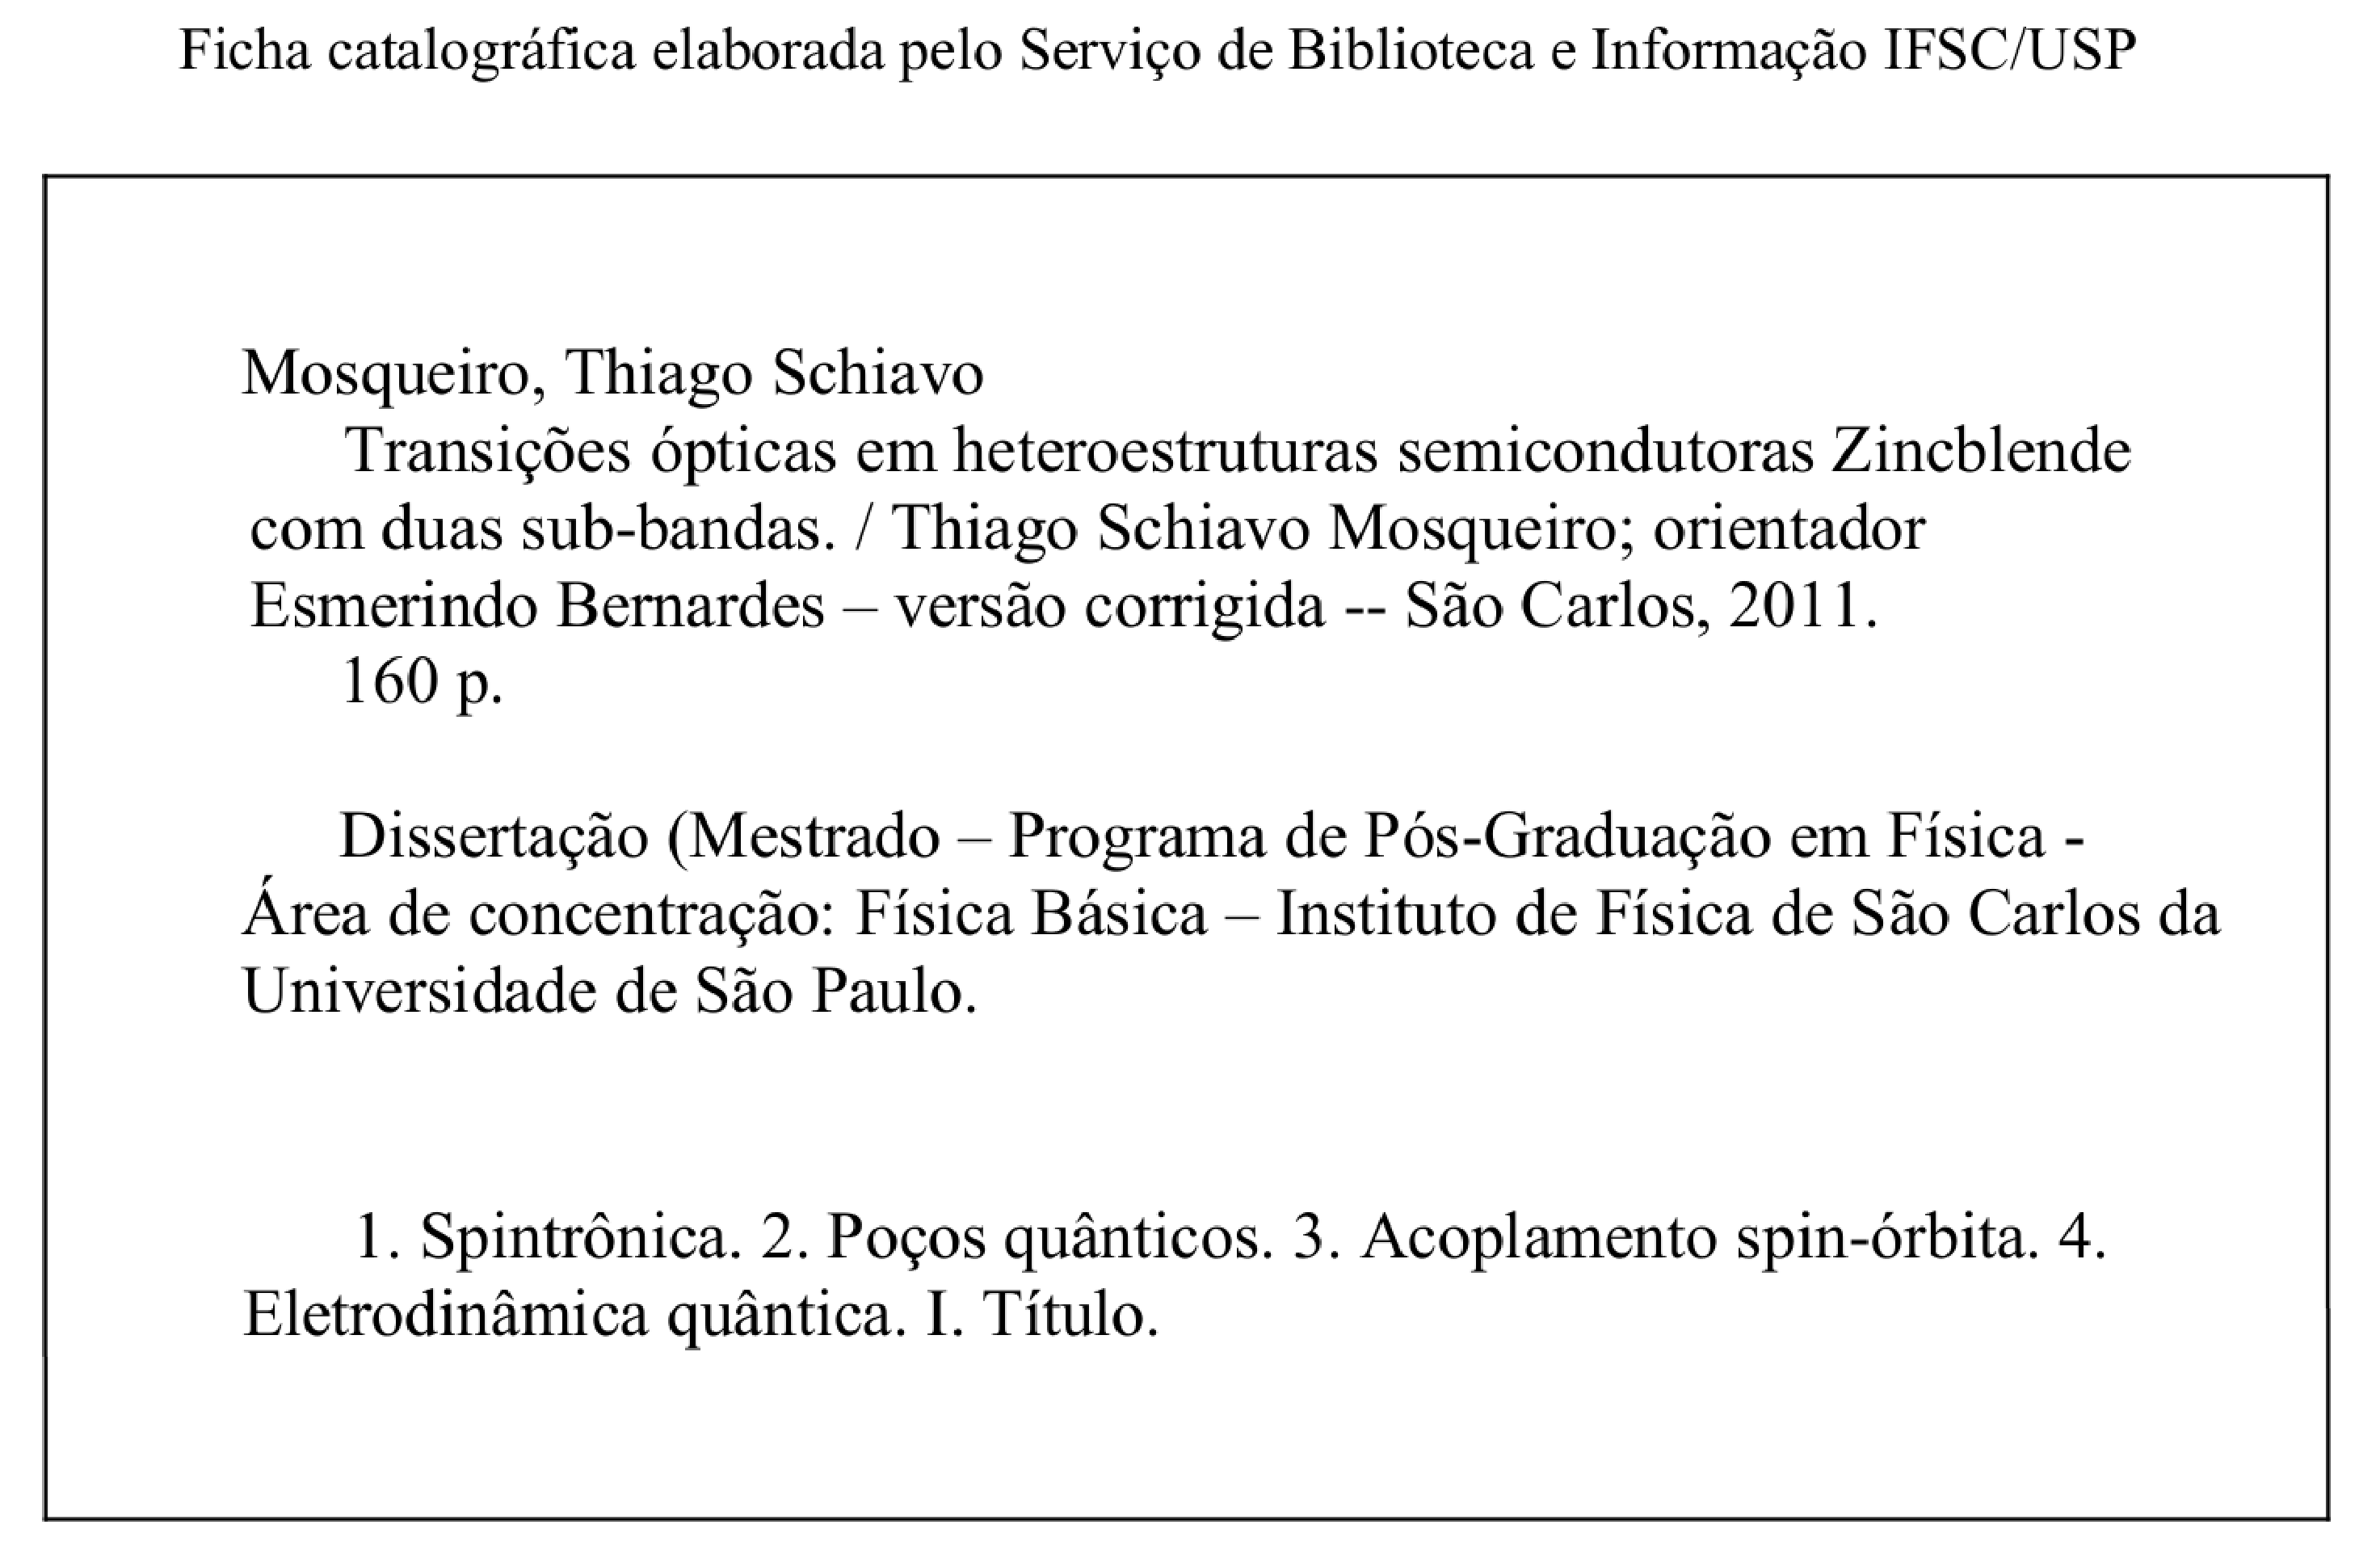
\includegraphics[scale = 0.28]{fichacatalografica}
  \end{center}
\end{center}


% \begin{folhadeaprovacao}
% Disserta��o apresentada ao Programa de P�s-Gradua��o em F�sica do Instituto de F�sica de S�o Carlos da Universidade de S�o Paulo, para obten��o do t�tulo de mestre em Ci�ncias.
% 
% \assinatura{Prof. Dr. Esmerindo de Sousa Bernardes\\ Orientador}  
% \assinatura{Prof. Dr. Iouri Poussep\\ Instituto de F�sica de S�o Carlos -- Universidade de S�o Paulo}
% \assinatura{Prof. Dr. Marcel Novaes\\ Departamento de F�sica -- Universidade Federal de S�o Carlos}
% \end{folhadeaprovacao}